\section{Core-periphery structure}

Previous research on Stack Exchange communities have attempted to explain how different types of users interact. In Question-Answer communities are expected popular and casual users \cite{santos2019activity, santos2019self}. Popular users generate the majority of interactions in the system, they are experts in community and take care on answering questions and engage the discussions through comments. As popular users they considered the $10 \%$ of the most active users, and showed that popular users are highly connected not only among themselves but also with casual users.

We tested this theory on all eight communities. We focused on 30 days sub-networks and showed how the number of links per node among popular users and between popular and casual users, evolve over time, figure \ref{fig:pop_cas_users}. We also compare active and closed communities of the same topic, so links per nodes in active sites are larger than in closed communities.

\begin{figure}[h!]
	\centering
	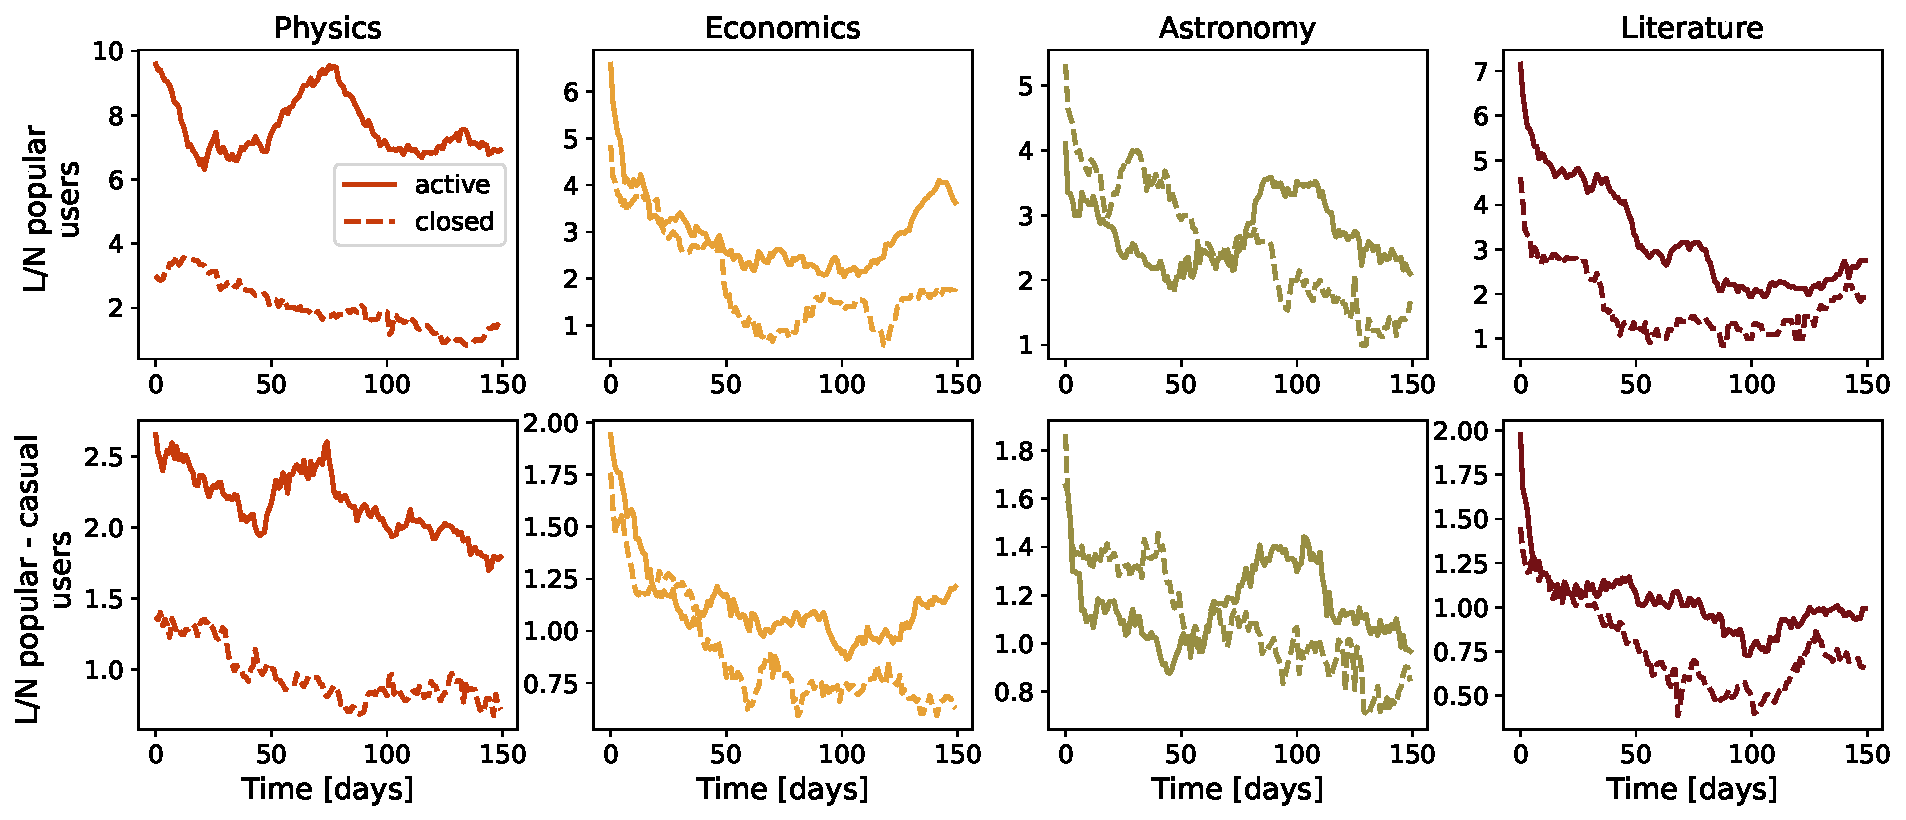
\includegraphics[width=\linewidth]{figures/stackexchange/popular_casual_users.pdf}
	\caption{Links per node among popular users (top 10\% of users) and between popular and casual users (everyone but popular users).}
	\label{fig:pop_cas_users}
\end{figure} 

Although, we find the difference between active and closed communities, the split according to $10\%$  most active users does not guaranty that all popular users will be considered. Furthermore, the smaller group of frequently active users is similar to the core users in core-periphery structure. This is why we are going to detect the core of the each 30day network. By this, separation is based on the network structure, and is more consistent, as using algorithmic approach we optimize the connectivity inside the core, periphery and among them. Core-periphery structure has core that is densely connected group of nodes, while the periphery has low density \cite{fortunato2010community, gallagher2020clarified}. 

We use Stochastic Block Model (SBM) to infer the core-periphery structure of each 30 days network snapshot and analyses how core structure evolve over time.  The  SBM algorithm is adapted for inferring the core-periphery structure, \cite{gallagher2020clarified}. For each 30 days network we run the sample of 50 iterations and choose the model parameters according to minimum description length. As stochastic models start from the random configuration, they can converge to different states, so we analyzed the stability of the inferred structures. More details are given in the appendix. We found that obtained structures differ, but minimum description length does not fluctuate too much. Also, different similarity measures between inferred core configurations take values higher than 0.9, indicating that core structure is stable. 

Number of users in core of active communities is higher than in closed communities, top panel on figure \ref{fig:core_size}. On the other hand we do not find strong difference between the fraction of core users in the closed and active communities. Furthermore, the fraction of users in core differ from the $10\%$, and it is constantly changing, bottom panel \ref{fig:core_size}. 

\begin{figure}[h!]
	\centering
	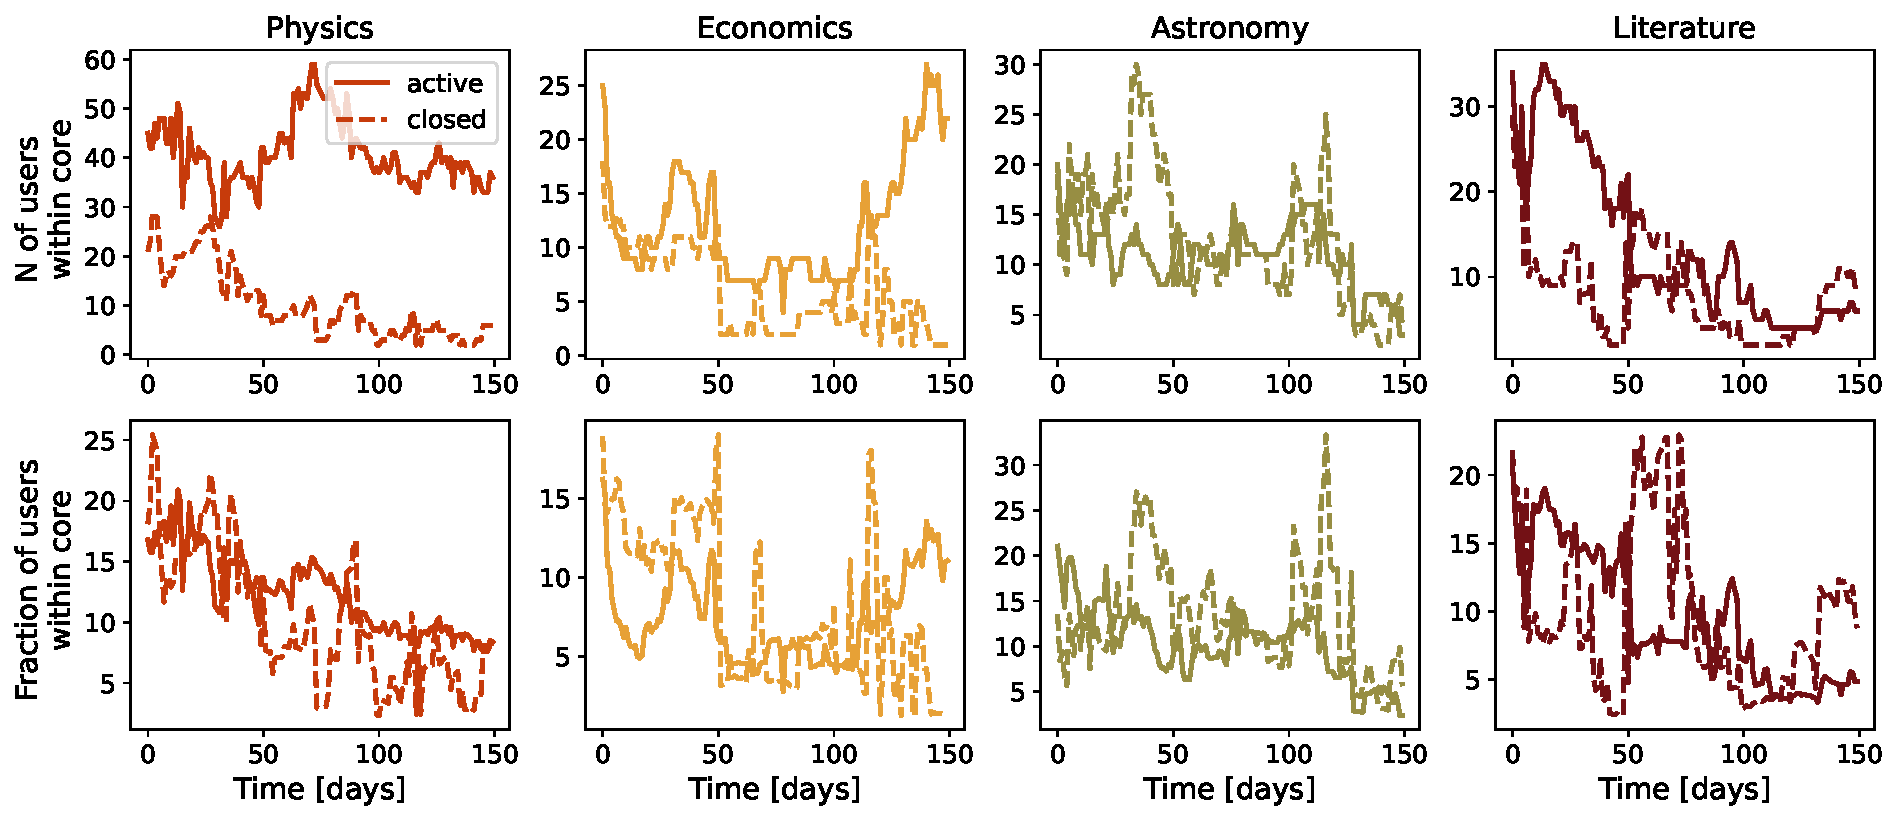
\includegraphics[width=\linewidth]{figures/stackexchange/core_users.pdf}
	\caption{Just for reference size of the core (top) and fraction of users in core (bottom). Solid lines - active sites; dashed lines - closed sites.}
	\label{fig:core_size}
\end{figure}

The number of users is constantly changing, but the remaining question is how much the core structure is stable. We compute the Jaccard's coefficient between core users in networks at time points $t_1$ and $t_2$. The Jaccard coefficient range from 0 to 1, so the larger values of Jaccard index indicate the more similar cores. 
The highest values are found around diagonal elements where we compare networks closer in time, see figure \ref{fig:jaccard_hm}. The core membership is changing over time, and it is more frequent in the closed communities. 

\begin{figure}[h!]
	\centering
	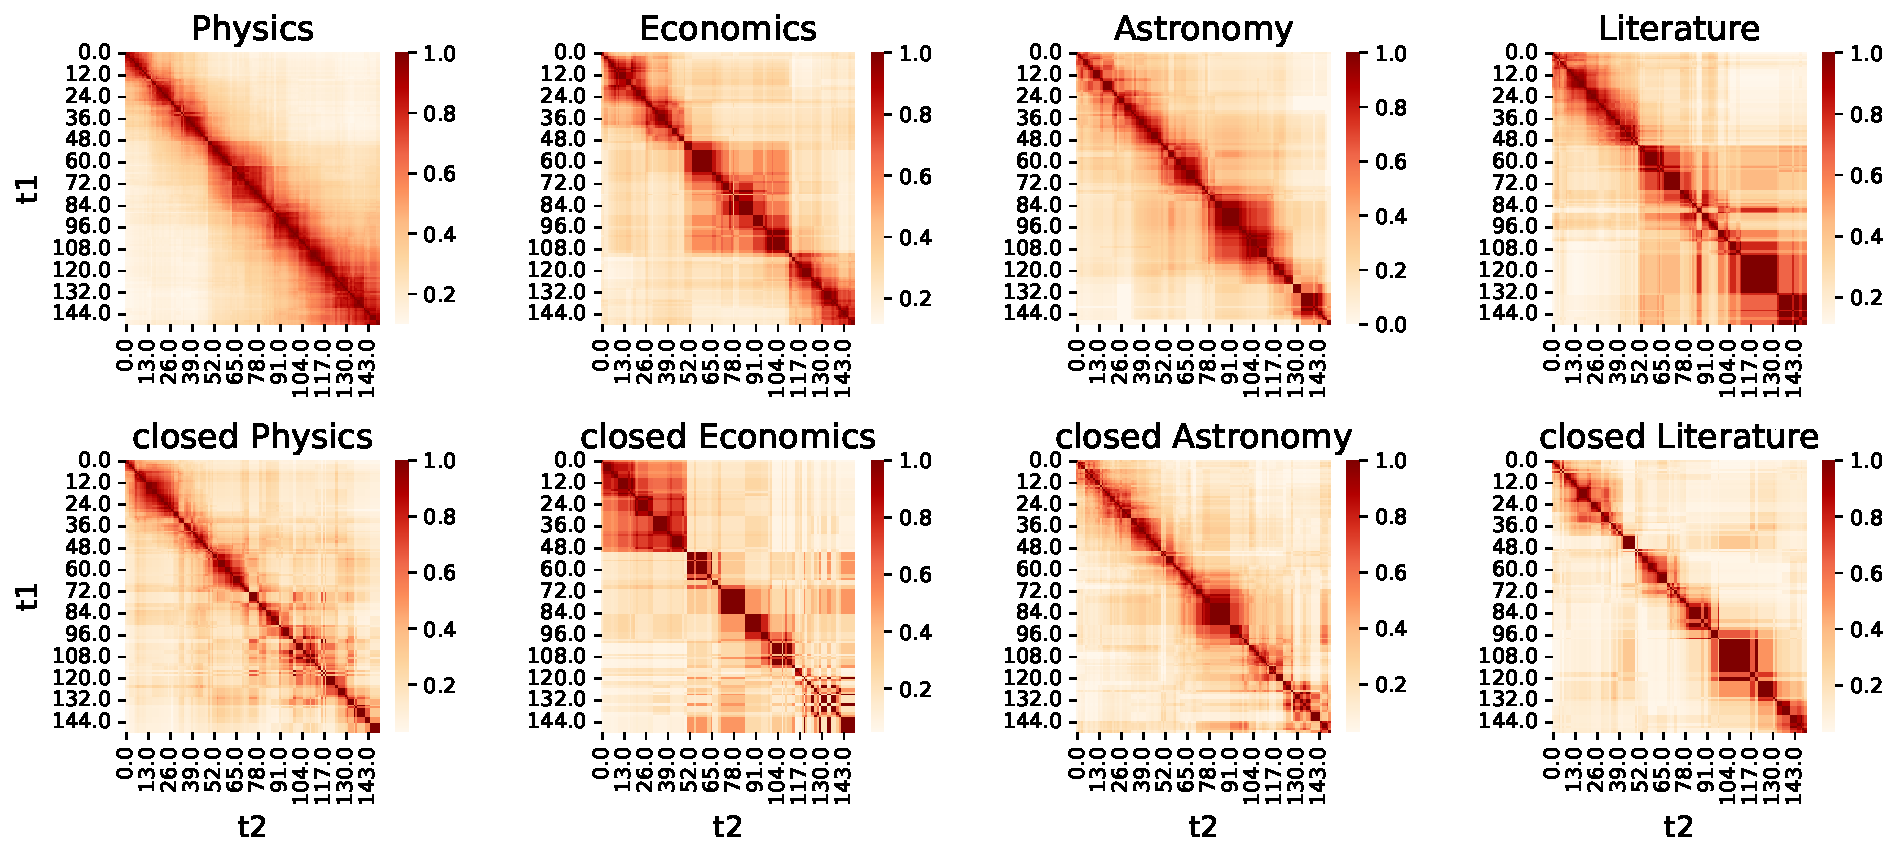
\includegraphics[width=\linewidth]{figures/stackexchange/jaccard_heatmap.pdf}
	\caption{Jaccard index between core users in  sub-networks at time points $t1$ and $t2$}
	\label{fig:jaccard_hm}
\end{figure}  

The average Jaccard index between cores in networks separated by time interval $t_i-t_j$ with the standard deviation confidence interval are shown in figure \ref{fig:jaccard_mean}. The Jaccard index decreases with relative time difference between networks faster in closed communities. The relatively high overlap between distant networks confirms that active networks have more stable core. 

\begin{figure}[h!]
	\centering
	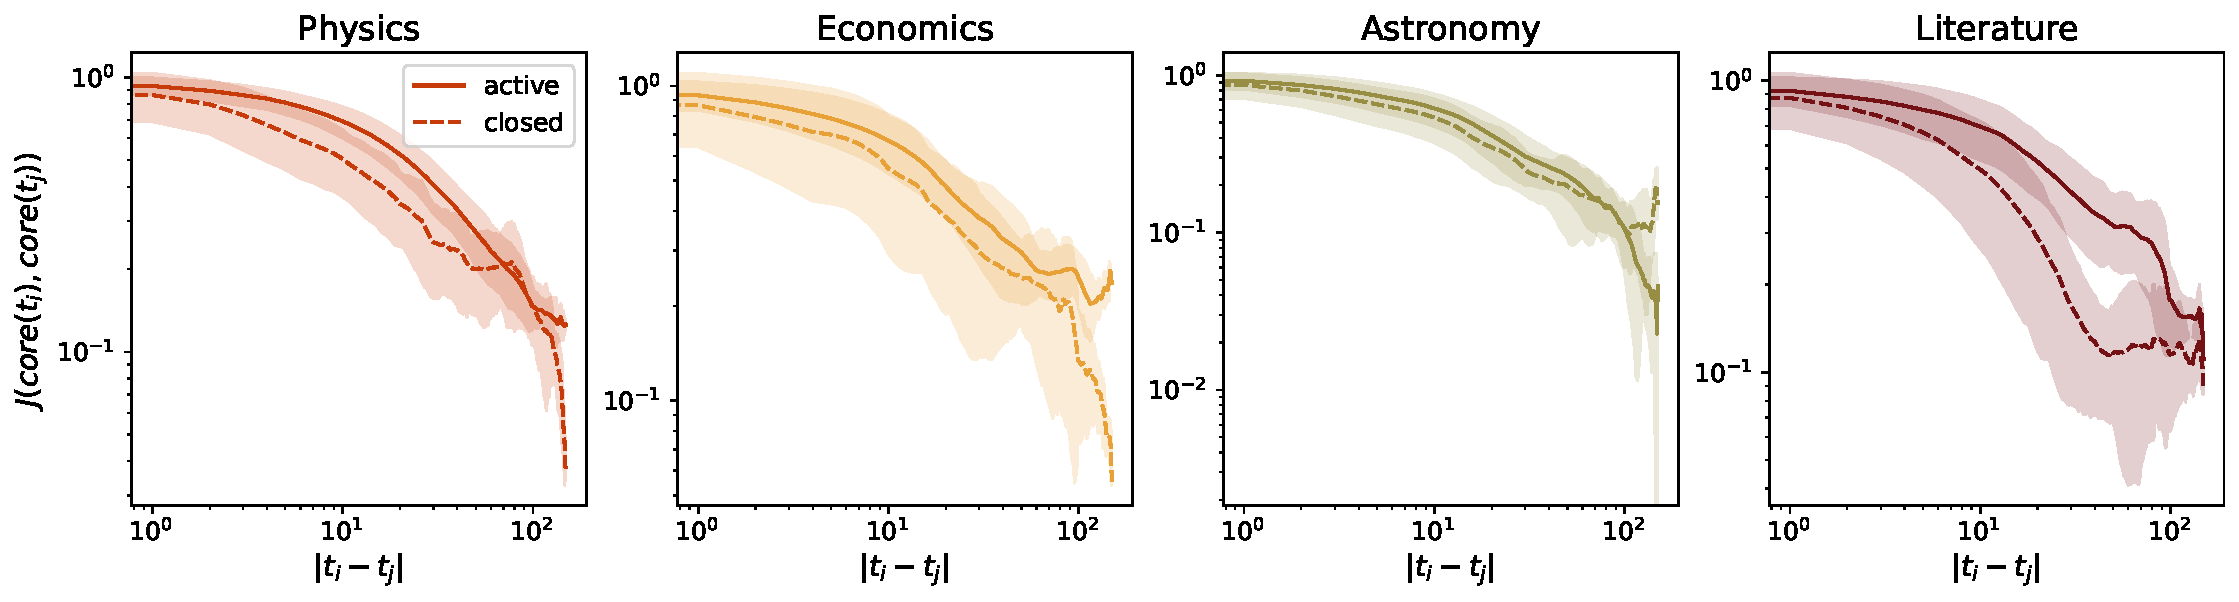
\includegraphics[width=\linewidth]{figures/stackexchange/jaccard.pdf}
	\caption{Jaccard index between core users in 30days sub-networks for all possible pairs of 30 days sub-networks separated by time interval $|t_i - t_j|$}
	\label{fig:jaccard_mean}
\end{figure}

Finally, we examine how the connectivity of the users in the core and between core and periphery evolve over time. On figure we show the $L/N$ in the core, that is proportional to the average degree of the network $2L/N$. The Physics community has more than twice larger connectivity than closed Theoretical Physics. For Literature we also find higher connectivity, but at the end of observation period the values become, the connectivity in active site drops and becomes similar as in closed one. For Economics and Astronomy the difference between active and closed site is not so clear. At the beginning of the period for the sites on economic topic, connectivity is similar, After 50 days of community life, connectivity in active communities is starting to rise, while in the case of closed economics it is dropping. For Astronomy, the connectivity is higher in closed communities, in the first 50 days, After this, period we find the sudden rise in the connectivity of active astronomy, but again it is dropping and becomes comparable to the connectivity values in closed site. The similar conclusions can be drawn for the connectivity between core and periphery. The largest difference between active and closed site is observed for Physics.  When it comes to active communities that are still in the beta phase, they either have the same core-periphery connectivity as their closed counter part, or as in the case of Astronomy, their periphery is weaker connected to the core during the first 50 days of their life, see Fig. \ref{fig:links_per_node}. 

\begin{figure}[h]
	\centering
	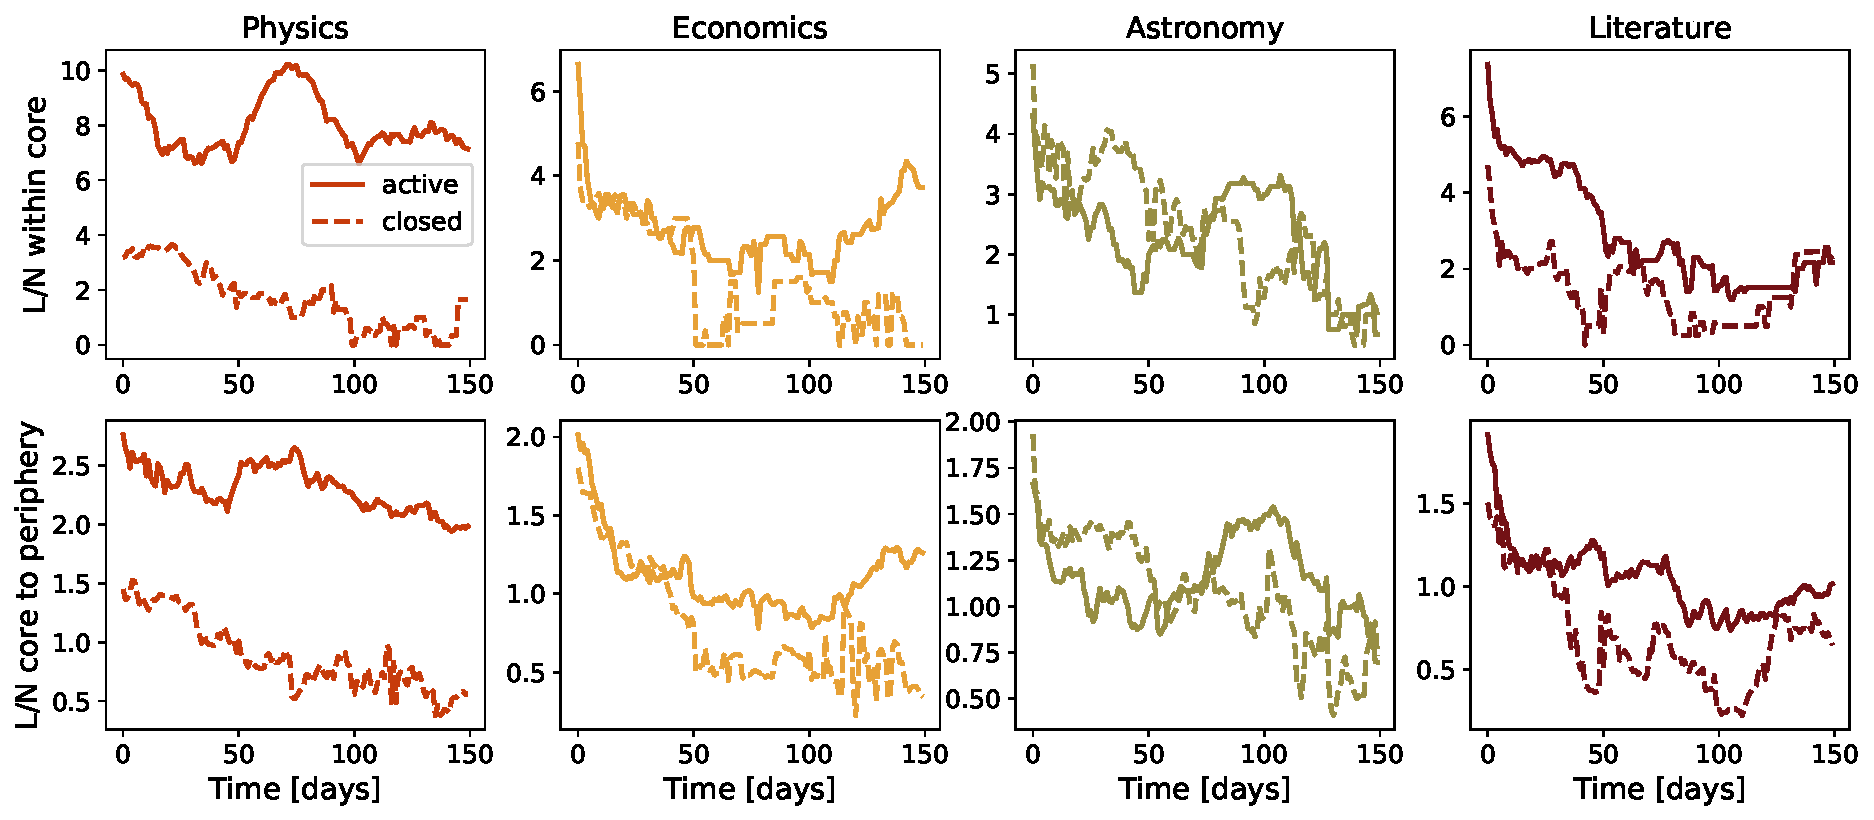
\includegraphics[width=\linewidth]{figures/stackexchange/core_connectivity.pdf}
	\caption{Links per node in core and links per node between core and periphery.}
	\label{fig:links_per_node}
\end{figure}

